% PLEASE FOLLOW POSTED GUIDELINES!!

% Please see the two LAr CDR 'guidelines' writeboards in basecamp
% at https://lbne-doc.basecamphq.com/projects/4264323/writeboards
% One is for text, the other for images and figures 

% Replace the following when the name of the experiment is decided
\newcommand{\LBNE}{LBNE}
\newcommand{\COMPARTMENT}{detector section}
\newcommand{\COMPARTMENTS}{detector sections}

%%%%%%%%%%%%%%%%%%%%%%%%%%%%%%%%%%%%%%%%%%%%%%%%%%%%%%%%%%%%%%%%%%%%%%%%
%%%%%%%%%%%%%%%%%%%%%%%%%%%%%%%%%%%%%%%%%%%%%%%%%%%%%%%%%%%%%%%%%%%%%%%%
\chapter{Data Acquisition}
\label{ch:trig}

The data acquisiton (DAQ) subsystem provides the data collection
in a robust fashion and optimized for the specific needs of the neutrino and
underground physics of the experiment.  The scope includes design,
procurement, fabrication, testing, delivery and installation of a
combination of custom and commercial electronics modules, (including
commodity computing and networking hardware), as well as both
commercial and internally developed software.

The \LBNE\ DAQ must collect data from (a) interactions which are
associated with the beam, (b) high energy ($>100$~MeV) interactions
which are asynchronous such as atmospheric neutrinos, proton decay,
cosmic ray muons etc., and (c) low energy interactions such as those
from diffuse supernova neutrinos or a possible supernova explosion in
our galaxy.  For case (a) and (b), it is essential to record the
maximum information about each event --- the current design presented
allows collection of all the LArTPC data with no zero suppression
whatsoever.  For supernova physics, it is essential to have the
maximum possible uptime, to be sure data is being collected when a
supernova occurs.
The sensitive time needed for a supernova is at least 10 seconds,
during which the data flow will increase dramatically, and zero
suppression of some form will be required.  The design follows many of
the principles of other neutrino and collider experiments with scope
for a multi-level trigger and continuous readout to cope with events,
such as atmospheric neutrinos, that are asynchronous with the beam.

An innovation of the \LBNE\ DAQ is a modular DAQ design,
as described in section~\ref{sec:daq_upper}, which extends the
modularity of the \LBNE\ far detector design and facilitates both
staging and a possible distributed (worldwide) approach to design and
procurement.   It allows the different \COMPARTMENTS\ to be
operated independently, and in so doing allows an added degree of
robustness to data collection, in particular supernova burst
detection, by giving a method for eliminating entirely even short
periods when the entire detector is off.  It also allows for unique 
design features to be possible in the different \COMPARTMENTS\ 
of \LBNE.

The majority of this chapter describes the full conceptual design for
the main data acquisition which could be used in all, or just some of
the \COMPARTMENTS\ of the experiment.  This is the reference design,
used in the 2015 cost and schedule estimations for \LBNE.  

%% Remove the following to keep it crisp
%There is scope for modification and improvements to this conceptual
%design, however we believe that the one presented here satisfies the
%requirements for the experiment and so gives a realistic indication
%that it is feasible and of the cost.  Further innovation to increase
%robustness or performance is welcome, and the modular DAQ design allows for
%sufficient modularity that innovations can also be added to the later
%\COMPARTMENTS\ after the initial \COMPARTMENTS\ are deployed.

The main data acquisition is introduced in
section~\ref{sec:daq_intro}.  It is comprised of a readout for the
LArTPC based on COB modules (section~\ref{sec:daq_cob}), a readout for
the photon detectors based on SSP modules (section~\ref{sec:daq_ssp}),
a time synchronisation system (section~\ref{sec:daq_time}) and a
readout and trigger generator for auxiliary signals associated with
the experiment (section~\ref{sec:daq_penn}).  The real time data
collection is performed by a toolkit called artDAQ
(section~\ref{sec:daq_artDAQ}) that will implement two arms of data
collection, event-building and processing; 
one of these is primarily dedicated to collection of full non-zero
suppressed data for the most important triggered events such as beam
or atmospheric neutrino candidates;  the other arm receives
zero-suppressed data from the whole detector for all times, it is responsible for
deadtimeless triggering in software of these important events, has ring-buffers to
store potential supernova events, and records low energy physics events.
The run control
(section~\ref{sec:daq_runcontrol}), online monitoring
(section~\ref{sec:daq_om}), slow control
(section~\ref{sec:daq_slowcontrol}) and infrastructure for the DAQ
subsystem (section~\ref{sec:daq_infrastructure}) are also described.
There follows the description of the modular DAQ design approach
as introduced above, in section~\ref{sec:daq_upper}.  This allows a
heterogeneous approach to different \COMPARTMENTS\ of the DAQ and
gives the ability to keep the majority of the detector running when
one part needs to stop data taking for maintenance.

\section{Introduction}
\label{sec:daq_intro}

\subsection{System overview} 

The DAQ subsystem will perform the primary functions of:

\begin{itemize}
  \item Readout of raw data from the LArTPC electronics and the photon
    detector subsystem,

  \item Continuous filtering and assembly of data to be treated
    offline as individual events, including receiving and using the
    Fermilab beam-spill signal, 

  \item Logging data to persistent storage media,

  \item Configuration, online calibration/checkout, and control of 
        operations of detector electronics, including the generation 
        and distribution of timing and control signals,

  \item Control of, and readout of data from, devices 
        providing real-time information on detector, subsystem 
        and environmental conditions, and  

  \item Providing user/operator interfaces for these functions via 
        a run control system.
\end{itemize}

A reference design for the DAQ subsystem is presented in this chapter.
The development of this design is guided by recent experience gained
in the development of relevant systems for the MINOS,
NO$\nu$A~\cite{novatdr} and MicroBooNE~\cite{microboonecdr}
experiments, as well as from experiments with comparable channel
counts and/or experimental conditions, such as D-Zero, CDF, NA48 and
ICARUS.  Guidance and experience is also available from the design and
operation of the LBNE 35t prototype and the future CERN testing
program.

The DAQ subsystem is to be located external to the cryostat vessel,
with components in the detector halls (sharing rack space near the
cryostat feedthroughs with the photon readout, and the power supplies
for components inside the cryostat) and in an underground computer
room for the trigger and data collection computers.  A small computer
room on the surface will also be required for GPS units and network 
connections between the fiber underground and the network to connect 
to Fermilab.  It is not decided yet whether a larger control room or 
computer room on the surface is needed in addition to the one underground. 
The interfaces to this work package are with the front-end electronics for the LArTPC, the
photon-detector subsystems and the offline computing.  

To increase
robustness and up-time, the modular DAQ design concept makes a
comparatively loose coupling between the DAQ subsystems in each
detector hall, to allow calibration or maintenance to proceed in one,
while data collection continues in the others.  The DAQ subsystem
includes the run of optical fibers to the surface for transfer of data,
GPS time synchronisation and e.g. telephone.  The DAQ subsystem
interfaces with the Fermilab Accelerator complex (the beam-spill
signal), and has a read-only interface with the cryogenics subsystem
for logging of conditions.  

\begin{cdrfigure}[DAQ subsystem block diagram]{daq15_main}{Block diagram layout of the main
    components of the DAQ subsystem.}
\begin{tikzpicture}[
  every matrix/.style={ampersand replacement=\&,column sep=0.4cm,row sep=0.6cm},
  to/.style={->,>=stealth',shorten >=1pt,semithick,font=\sffamily\footnotesize},
  data/.style={thick},
%  box/.style={draw,thick,rounded corners,fill=yellow!20,inner sep=.3cm},
  box/.style={draw,inner sep=.1cm},
  boxa/.style={box,align=center}]

% Lay the nodes out using a matrix
  \matrix{   
% 1st row
  \node[boxa] (ce) {Cold\\Electronics};
 \&
 \& \node[boxa] (rce) {RCE\\LArTPC data\\processors};
 \&
 \& \node[boxa] (trigfe) {Trigger\\frontend\\Computers};
 \& \node[boxa] (trigbe) {Trigger\\backend\\Computers}; \\

% 2nd row
 \& \node[box,inner sep=0.4cm] (fthru) {}; 
 \& \node[boxa] (time) {Time\\Sync};
 \&
 \& \node[boxa] (sc) {Slow\\Control};
 \& \\

% 3rd row
  \node[boxa] (pd) {Photon\\Detectors};
 \&
 \& \node[boxa] (ssp) {SSP\\Photodetector\\digitizers};
 \&
 \& \node[boxa] (datafe) {Data\\frontend\\Computers};
 \& \node[boxa] (databe) {Data\\backend\\Computers}; \\
 };

\coordinate (fthruWL) at ($ (fthru.south west)!0.3!(fthru.north west) $);   % West Low edge of fthru 
\coordinate (fthruWH) at ($ (fthru.south west)!0.7!(fthru.north west) $);   % West High edge of fthru 
\coordinate (fthruEL) at ($ (fthru.south east)!0.3!(fthru.north east) $);   % East Low edge of fthru 
\coordinate (fthruEH) at ($ (fthru.south east)!0.7!(fthru.north east) $);   % East High edge of fthru 

\coordinate (trigfeWL) at ($ (trigfe.south west)!0.3!(trigfe.north west) $);   % West Low edge of trigfe 
\coordinate (trigfeWH) at ($ (trigfe.south west)!0.7!(trigfe.north west) $);   % West High edge of trigfe
\coordinate (datafeWL) at ($ (datafe.south west)!0.3!(datafe.north west) $);   % West Low edge of datafe
\coordinate (datafeWH) at ($ (datafe.south west)!0.6!(datafe.north west) $);   % West High edge of datafe

\coordinate (rceEL) at ($ (rce.south east)!0.3!(rce.north east) $);  % East low edge of RCE 
\coordinate (rceEH) at ($ (rce.south east)!0.7!(rce.north east) $);
\coordinate (sspEL) at ($ (ssp.south east)!0.3!(ssp.north east) $);  % East low edge of SSP
\coordinate (sspEH) at ($ (ssp.south east)!0.8!(ssp.north east) $);

\coordinate (rceSR) at ($ (rce.south)+(0.7cm,0) $);  % South right edge of RCE 
\coordinate (sspNR) at ($ (ssp.north)+(0.7cm,0) $);  % North right edge of RCE 
\coordinate (scWL) at ($ (sc.south west)!0.3!(sc.north west) $);  % West low edge of SC 
\coordinate (scWH) at ($ (sc.south west)!0.7!(sc.north west) $);  % West high edge of SC 

\draw[data] (ce) -| ($(fthruWH)-(0.1cm,0)$) -- (fthruWH);
\draw[data] (pd) -| ($(fthruWL)-(0.1cm,0)$) -- (fthruWL);
\draw[data] (fthruEH) -- ($(fthruEH)+(0.1cm,0)$) |- (rce);
\draw[data] (fthruEL) -- ($(fthruEL)+(0.1cm,0)$) |- (ssp);

\draw[data] (rceEH) -- ($ (rceEH)+(0.5cm,0) $) |- (trigfeWH); 
\draw[data] (rceEL) -- ($ (rceEL)+(0.5cm,0) $) |- (datafeWH); 
\draw[data] (sspEH) -- ($ (sspEH)+(0.55cm,0) $) |- (trigfeWL); 
\draw[data] (sspEL) -- ($ (sspEL)+(0.55cm,0) $) |- (datafeWL); 

\draw[data] (trigfe) -- (trigbe);
\draw[data] (datafe) -- (databe);

\draw[data,dashed] (time) -- (rce);
\draw[data,dashed] (time) -- (ssp);

\draw[data,dashed] (scWH) -| (rceSR);
\draw[data,dashed] (scWL) -| (sspNR);

\draw[data,dotted] (fthru.north) -- ($(fthru.north)+(0,2.7cm)$) node [left] {In cryostat} node [right] {Room temp.};
\draw[data,dotted] (fthru.south) -- ($(fthru.south)-(0,2.7cm)$);

\end{tikzpicture}
\end{cdrfigure}
The DAQ subsystem reference design described in this chapter is shown
in figure~\ref{fig:daq15_main} and consists of the following
components:
\begin{itemize}
  \item Logic and processing elements called ``Reconfigurable cluster
    elements'' (RCE) residing on daughter cards in ATCA crates located
    in the detector hall to receive data from the LArTPC.  These carry
    out data merging, buffering and compression and transmission to the
    local farms of commodity computers (see section~\ref{sec:daq_cob})
  \item custom `SSP photon detector digitizers' which digitize and
    process the light signals (described in section~\ref{sec:daq_ssp}) 
  \item two local farms of commodity computers providing two separate
    branches of readout, triggering, event processing and logging of the
    detector computers; these use the artDAQ toolkit for data
    acquisition systems (see section~\ref{sec:daq_artDAQ})
  \item a custom timing system consisting of a master unit, situated
    on the surface, that locks onto a GPS clock and distributes timing
    signals to the data concentrator modules via slave units (see
    section~\ref{sec:daq_time})
  \item dedicated computer nodes that host run control, online
    monitoring, database services and slow controls processes
\end{itemize}
%
The DAQ subsystem does not include power-supply hardware for the
LArTPC or front-end electronics, nor does it include the cryogenics
subsystem process-control and monitoring functions.  The SSP readout
modules for the photon subsystem is in the photon subsystem part of
the project.

\subsection{Physics Considerations}
\label{sec:daq_phys}

The physics considerations determine the scale of the primary tasks of
digitising the LArTPC data readout, merging the photon system data,
event building and online processing.  In addition to rates for
processes of interest, the DAQ subsystem design depends critically on
the specifications for the LArTPC and front-end electronics systems,
chosen to satisfy the \LBNE\ physics requirements.  The sampling rate
of 2~MHz has been chosen so as to achieve the required position
resolution along the ionisation drift direction. Obtaining sensitivity
to signals that occur independently of the \LBNE\ beam spill, such as
those from nucleon decay, atmospheric neutrinos or supernova-neutrino
bursts, requires a free-running transmission of data from the LArTPC
front-end electronics.  In principle, this same technique can be used
to collect the beam events as well, however we will supplement the
robustness of the beam data collection by transferring knowledge of
the spill times from Fermilab to the far detector site using GPS.

The task of data transfer is facilitated by multiplexing and utilizing
high-speed data lines (1Gbps) in front-end ASICs in the LAr, and by
%redundant (Discussed with Jim, decided to drop this word) 
data lines that
provide connection to data-acquisition hardware located outside the
cryostat.  The hardware receiving the raw TPC data then perform
zero-suppression and/or data compression, as desired.  A challenge in
real-time is to use the information of the channels which have hits on
them in a particular interaction to determine a larger set of
channels, which including the surrounding ones, that should be read
out.  The design, as depicted in figure~\ref{fig:daq15_main},
addresses this difficulty by using two data paths.  The trigger data
path continuously receives the data from the channels that the online
hardware determines have hits on them.  This determines whenever an
event occurs and designates regions of interest which are to be read
out in more detail.  Ring buffers in the RCEs store the non-zero
suppressed data until the region of interest information is received,
at which point they transmit non-zero suppressed data to the second
path, the Data path which reads out the interesting events (all
candidates of cosmic rays, beam events, atmospheric neutrinos, proton
decays etc.) for all channels within active APAs with no zero
suppression within the entire event drift window period.  This allows
the maximum available information for these, the most important \LBNE\
events, to be recorded for offline analysis using e.g.\ Fourrier
transform deconvolution techniques.

The trigger data path handles all the zero suppressed data and can
store it for long periods, either in ${\cal O}(\mathrm{hours})$-long
ring buffers or in permanent offline storage for collection of data
from a supernova neutrino burst.  Experience from MicroBooNE, which
has a similar division of lossy-compressed and lossless-compressed
data readout, will be vital in optimising this feature of the data
acquisition.  During a supernova neutrino burst, the data path may
also be used for data collection, the optimum way for utilising this
is still to be studied.

In addition to physics considerations, the DAQ design goals include
minimizing the impact of single-point failures, maximizing the uptime
and maximizing the use of commercial components.  The robustness is
addressed in part by some redundancy (and ability to cross-check)
between the two arms of data transfer shown in
figure~\ref{fig:daq15_main}, and by the separation of sub-system
control in different \COMPARTMENTS\ of the experiment
(section~\ref{sec:daq_upper}).

\subsection{Event Rates and Timing}
\label{sec:v5-daq-assumptions}

For the reference design described here, sited at the 4850L of the Sanford Laboratory, the 
atmospheric-muon rate is small enough -- 0.1~Hz within the full LAr-FD active 
volume -- to contribute only negligibly to the DAQ bandwidth requirement.
%For reference, the rate at the alternate 800L site 
%is estimated to be 500~Hz within the active volume.  

Signals associated with beam events will be localized within the
LArTPC and synchronous with discrete (${\cal O} (1\,s)$ rep rate)
beam-spill intervals spanning approximately $10\,\mu s$ and will take
${\cal O} (2\,ms)$ for the ionization drifting in the LArTPC to take place.
However other physics events of interest will occur at random times,
and can be dispersed throughout the TPC volume as in the case of
neutrino bursts from supernovae.  Other specific signatures, such as
very slow-moving magnetic monopoles ($\beta < 10^{-3}$) may involve
signals spanning sample times exceeding the ionization-drift time.
% Possible reference: Thron J.L. et al. PhysRevD.46.4846 (1992),
% url = {http://link.aps.org/doi/10.1103/PhysRevD.46.4846} 

Cosmic-ray muons dominate the physics rate, even at the proposed 4850L
site.  However, this rate is negligible with respect to noise sources.
The reference design proposed here would be capable of operation at
shallower depths, up to about the 800L, without significantly impacting
the design.

As described in section~\ref{sec:fe_arch}, the cold electronics for a
single Anode Plane Assembly will consist of twenty 128-channel
Front-End Readout Boards, each providing four digital inputs to the
RCEs.  The Front-End Boards will generate non-zero-suppressed data,
i.e.\ a constant data rate of (1.5 bytes/sample $\times$ 32 wires/link
$\times 2 \times 10^6$ samples/wire/s $=$) 96\,MB/s.

Radioactive decay 
from $^{39}$Ar and $^{85}$Kr in the LAr, and to a lesser extent from 
detector materials (U/Th/Co/K), is estimated to provide a
65-kHz/APA rate of activity of energy above about 300~keV (0.3 MIPs) 
but less than $\sim 5\,$MeV, while 
electronics noise (assuming 10:1 S/N for 1 MIP, and a threshold of 0.3 MIPs) 
will contribute a relatively low rate per APA of singles.  
The data rate from cosmic ray muons at the 4850 level is considerably
lower.  Table~\ref{tab:daq-signal-rates} provides a summary of these rate 
estimates.
%
\begin{cdrtable}[Rates and data sizes/rates for various processes.]
  {lcccc}{daq-signal-rates} {Per-APA estimates of rates and
    data sizes/rates for various processes.  Mbps denotes millions of
    {\it bits} per second.  Unless otherwise stated,
    estimated numbers of samples and data rates assume suppression of
    signals below 0.3 MIP.  `Inst.\ Data Rate' refers to the number of
    bits in a 2.3-ms long data block divided by this time interval,
    while `Avg.\ Data Rate' factors in the process rate.  A 12-bit ADC
    is assumed, and no allowance is made for data items such as
    time-stamp, etc.}
  
    {\bf Process} & {\bf Rate } & {\bf Samples}
                  & {\bf Inst.\ Data } & {\bf Avg.\ Data}  
                  \cr 
                  & {\bf (kHz/APA)}  & {\bf (per APA)}
                  & {\bf Rate (Mbps)} & {\bf Rate (Mbps)} \cr \hline
    Generic 2.3 ms interval 
                  & 0.43 & $1.06 \times 10^7$ 
                  & 55,000 & 55,000 
                  \cr 
                  (not zero-suppressed) & & & & \cr \hline
    Cosmic ray muons (4850L)
                  &  $6\times 10^{-7}$ & $5 \times 10^4$ 
                  &  260 & $1\times 10^{-4}$
                  \cr 
                  & & & & \cr \hline
%    Cosmic ray muons (800L)
%                  &  0.0034 & $5 \times 10^4$ 
%                  &  260 & 2.0 
%                  \cr 
%                  & & & & \cr \hline
    10 GeV EM shower 
                  &  --- & $1 \times 10^6$
                  & 5,200  & --- 
                  \cr
                  & & & & \cr \hline
    Radioactivity: $\gamma$: U/Th
                  & $\sim 1$ & 40
                  & 0.48  & 0.48
                  \cr
    \phantom{Radioactivity:} $\beta$: $^{39}$Ar, $^{85}$Kr
                  & 63 & 24
                  & 18  & 18
                  \cr
%                  & & & &  \cr 
                  \hline
    Electronics noise
                  & $\sim 1$ & 15 
                  & 0.2  & 0.2 
                  \cr 
                  (not common mode) & & & & \cr \hline
\end{cdrtable}

The conclusion from table~\ref{tab:daq-signal-rates} is that the
average data rates out of the front-end electronics system are
manageable: about 20 Mbps of `salt and pepper' per APA due to
radionuclides in the Ar and LArTPC materials.  Large beam- or
atmospheric-neutrino interactions or showering ultra-high-energy
cosmic-ray muons will result in high (Gbps-level) instantaneous rates
on the scale of the maximum ionization drift period, but contribute
negligibly to the average rate.

\subsection{Architecture Summary}
\label{sec:v5-trig-daq}

The reference design of the DAQ system is summarized in block diagram
form in Figure~\ref{fig:daq15_main}.  Component counts are given in
Table~\ref{tab:daq15_component_counts}. 
%\todo{Update table.  Be precise and for what sized detector.}

\begin{cdrtable}[DAQ subsystem component counts]{ll}{daq15_component_counts}
  {DAQ subsystem component counts for one 10-kton module/cryostat.}
    {\bf Quantity} & {\bf Description} \\
   250  &  COBs (Cluster on Board) each with 8 RCEs,\\
   26  & 14-slot ATCA Shelves  \\
   27  & Ethernet Switches (one 10G, 26 1G)  \\  
   26  &  TPC Readout Compute Nodes \\
   1   &  Master Timing Unit with GPS Receiver\\
   27  &  Slave Timing Units \\
   11  &  Event Builder Compute Nodes \\
   8   &  Other computing nodes (server, run control, slow control etc)  \\
\end{cdrtable}

%%%%%%%%%%%%%%%%%%%%%%%%%%%%%%%%%%%%%%%%%%%%%%%%%%%%%%%%%%%%%%%%%%%%%%%%
%%%%%%%%%%%%%%%%%%%%%%%%%%%%%%%%%%%%%%%%%%%%%%%%%%%%%%%%%%%%%%%%%%%%%%%%
\section{TPC readout}
\label{sec:daq_cob}
%\subsection{COB - Cluster on board modules}

The primary interface between the TPC front-end electronics (FE) and
the DAQ subsystem consists of an ATCA-based system of RCEs
(Reconfigurable Cluster Elements).  The RCE system receives the
serialized raw data for the FE, stores it with no zero-suppression in 
ring buffers for later retrieval if a valid trigger is received, performs 
zero-suppression on it to send to the trigger-arm.  It packetizes and 
transmits the resulting data to the back-end
farms for event building and further processing.  Additionally,
the RCE system transmits timing and control signals to the FE as well
as forwarding configuration data to them at start-up.

\begin{figure}[hbt]
\begin{center}
\begin{tikzpicture}
\node[inner sep=0pt] (russell) at (0,0)
    {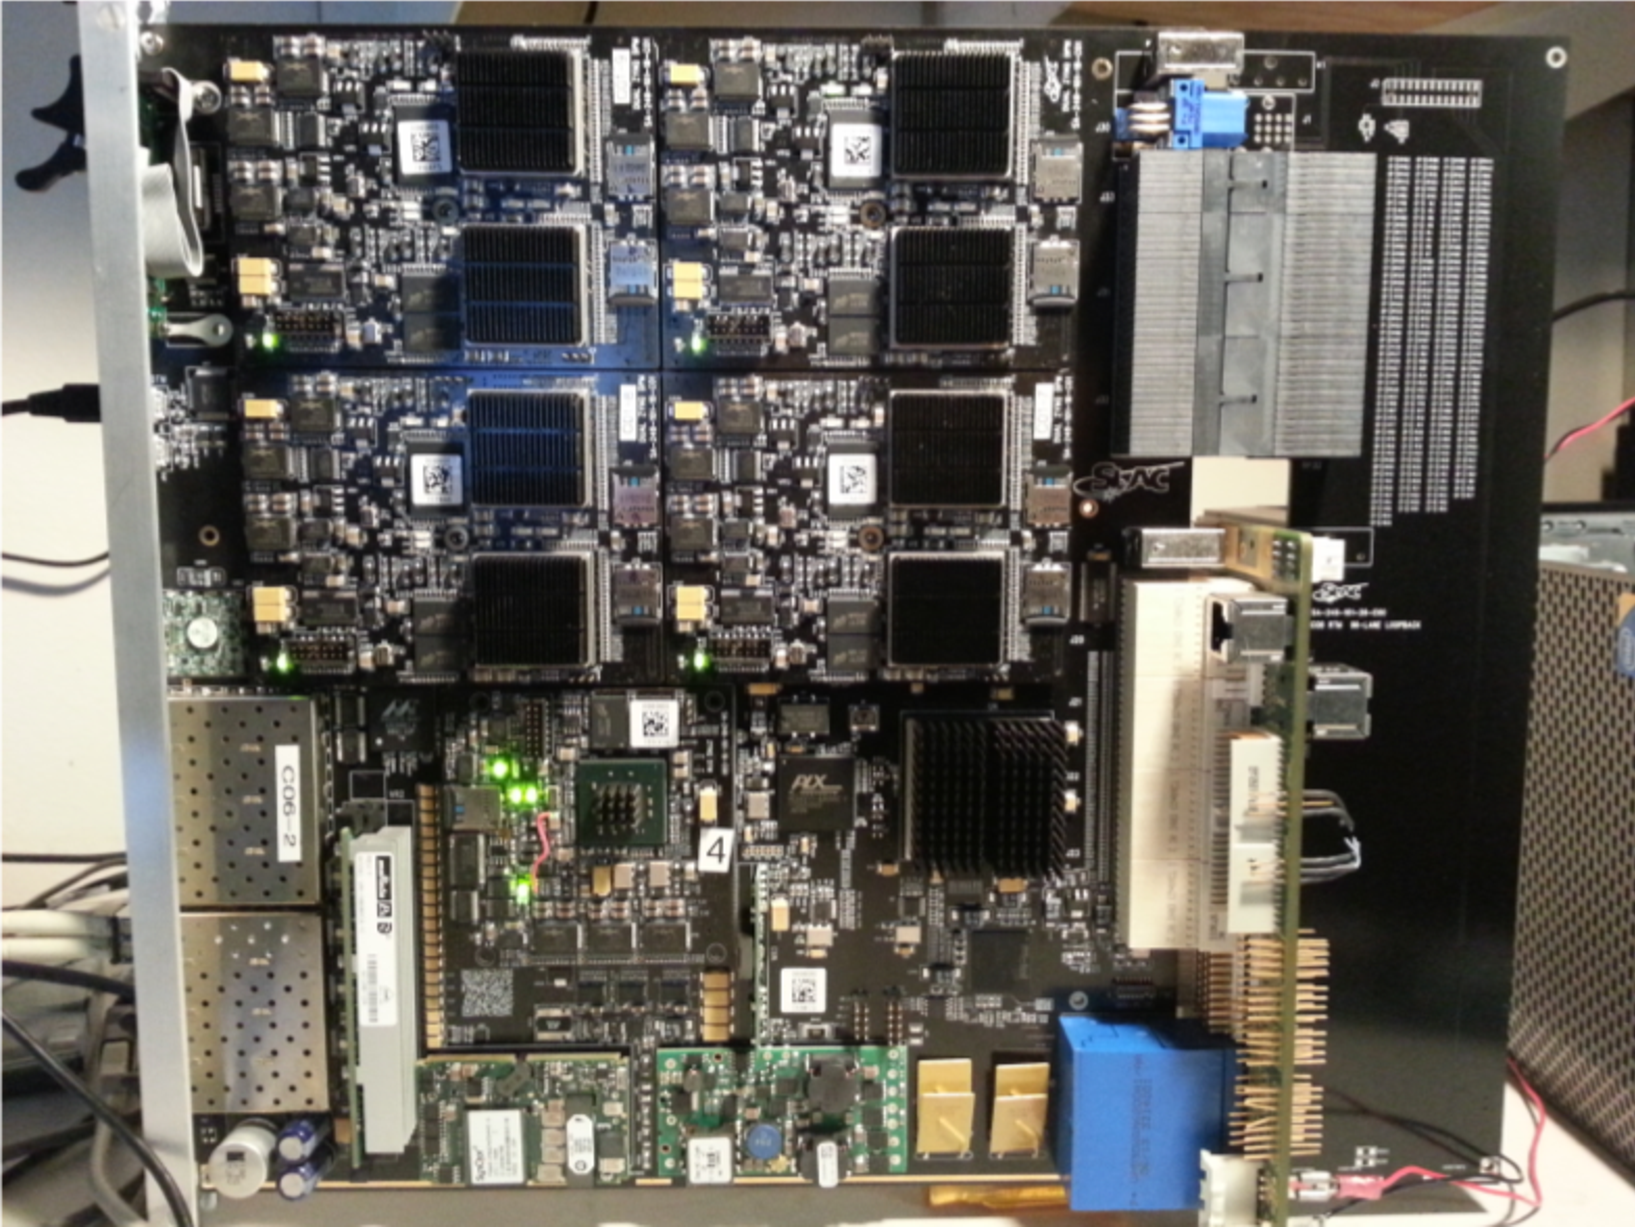
\includegraphics[scale=0.5]{daq15_COB-gen3.pdf}};
\draw[ultra thick] (russell.south west) ++(1.2,-0.2) -- node[below] {COB board} ++(9.5,0.);
\draw[ultra thick] (russell.south west) ++(10.9,-0.2) -- node[below] {RTM board} ++(2.,0.);
\end{tikzpicture}
  \caption{\label{fig:daq15_cob} The COB (left) and RTM (right). The eight black square units near the upper-left of the COB modules are the RCEs.}
\end{center}
\end{figure}
The RCE system consists the following components: a commercial ATCA
shelf (2-, 6-, or 14-slot), a Cluster-On-Board (COB) which is the
"front board" in ATCA terms, and a Rear-Transition-Module (RTM) which
is the "rear board".  The COB is a custom board, developed by SLAC,
which holds the processing power of the system.  The COB (see
Figure~\ref{fig:daq15_cob}) consists of 5 bays for holding daughter
boards, an onboard 10-GbE switch, and both 10- and 1-Gb ethernet
connections for communications with the back-end system.  Four of the
daughter-board bays are for Data Processing Modules (DPM), each of
which can hold up to two RCEs.  The RCE is the core processing unit of
the system; it is made up of a modern ``system-on-chip'' SoC (currently, the Xilinx
Zynq-7045) with multiple high-speed I/O ports (up to 10-Gbps each) and
1\,GBytes of external DRAM and flash memory controllers.  The
other bay on the COB contains the Data Transmission Module (DTM) which
is responsible for distributing timing and trigger information to and
between the DPMs.

While the COB hardware is application agnostic, the firmware and
software on the RCE and the RTM board are application specific. The
RTM provides the mechanical and electrical interfaces between the
front-end (or, in our case, the flange electronics) and the back-end,
as well as other external sources such as the timing or trigger
systems.  In the case of \LBNE,
fiber optic connections are used between
the flange and the TPC DAQ using QSFP+ connectors. This provides the required ground isolation.  These links are used for data transmission from the cryostat and also provide the synchronisation clock to run the ADCs.  Currently, each
RTM can accommodate up to 16 QSFP+ connections.

With 
%\todo{Erik suggests a simple diagram to accompany this paragraph} 
the assumption that each cold FE board multiplexes it's 128 wire
channels to 4 outputs at 1-Gbps each, the non-zero suppressed data for
1 APA can be fed into a single COB (containing 8 RCEs).  Each RCE
would receive data from 2 FE boards, perform zero-suppression, and
send the result to the trigger front-end computers.  There would also
be a large DRAM ring buffer to store a non-zero suppressed copy of the
data, which would be read out on request (see
figure~\ref{fig:daq15_main}) to the data front-end computers.

Figure~\ref{fig:daq15_atcapic} shows a COB in a two-slot ATCA shelf.
There are some options regarding the physical distribution of the
shelves.  One option is to have a smaller shelf at each flange port,
each shelf collecting data from the 2- or 4-APAs accommodated by that
port.  Alternatively, the fibers from all APAs could be routed to a
central location into a smaller number of large ATCA-shelves.

\begin{figure}[hbt]
  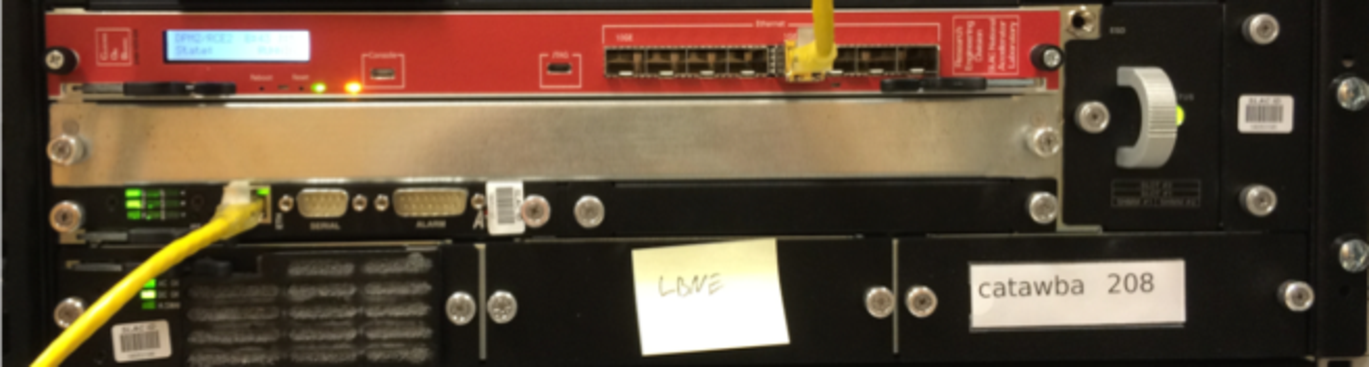
\includegraphics[scale=0.6]{daq15_acta-rtm.pdf}
    \caption{\label{fig:daq15_atcapic}A front view of the ATCA crate with a COB in the top slot. }
\end{figure}

%%%%%%%%%%%%%%%%%%%%%%%%%%%%%%%%%%%%%%%%%%%%%%%%%%%%%%%%%%%%%%%%%%%%%%%%
%%%%%%%%%%%%%%%%%%%%%%%%%%%%%%%%%%%%%%%%%%%%%%%%%%%%%%%%%%%%%%%%%%%%%%%%
\section{Photon detector readout}
\label{sec:daq_ssp}

The photon detection system is digitized and readout by a custom
module called the SIPM signal processor (SSP) which is described in
detail in section~\ref{sec_elec} in the photon detector chapter.
The module has ADC and signal processing hardware.  The output of the
SSP is Ethernet, interfaced with the same Xilinx Zynq architecture as
the COB which is used for the LArTPC data. The SSP therefore is able
to provide control, data and slow-control monitoring independently
from each other which facilitates a consistent interface between the
hardware and software parts of the DAQ.

%%%%%%%%%%%%%%%%%%%%%%%%%%%%%%%%%%%%%%%%%%%%%%%%%%%%%%%%%%%%%%%%%%%%%%%%
%%%%%%%%%%%%%%%%%%%%%%%%%%%%%%%%%%%%%%%%%%%%%%%%%%%%%%%%%%%%%%%%%%%%%%%%
\section{Timing System }
\label{sec:daq_time}

There are comparable requirements of \LBNE\ for timing with the NOvA
experiment.  That experiment uses a Global Positioning System (GPS)
receiver on the surface (in a module called the Master Timing Unit
(MTU) and a protocol that uses four twisted pair connections (on a
standard RJ45 connector) to fan out and then daisy-chain these signals
to the electronics.  We propose using the same concept with potential
enhancements and modernisation to distribute the timing from the
surface to the underground, among the readout modules for the photon
detector and also for distribution to the COBs for the LArTPC readout.
This will maintain a 64-bit counter synchronized to the absolute GPS
time on each of these readout modules.  In addition, we are using a
separate protocol for synchronisation of the cold electronics
boards from the counters on the COBs; this uses the same optical links
as the data path as described in section~\ref{sec:daq_cob}.  For
simplicity, this maintains a 64\,MHz clock, but not a large counter
synchronized on the cold electronics boards, the time being added when
the data reach the RCE.

The timing link is the only physical link other than the
communications network.  The system described here
provides several essential functions:
\begin{itemize}
\item Provides a time stamp so that data can be associated with a
  specific accelerator extraction cycle.
\item Provides a common 64 MHz clock to all front end electronics
  boards.
\item Synchronizes the data acquisition system so that all data from a
  given time period is sent to the same event builder.
\item Provides dynamic synchronization to the cold electronics so
  glitches in the clock signal are detected promptly.
\item Enables calibration and test pulses to be generated
  simultaneously for multiple channels.
\end{itemize}

\subsubsection{Beam triggers and time stamps}

A similar GPS based system will be used at Fermilab to record the times
of the accelerator spills which generate the 10\,$\mu$s bursts of
neutrinos.  There should be sufficient buffering in the trigger path
of the readout system shown on figure~\ref{fig:daq15_main} so that all
data can be buffered while the time stamp of the spill is
sent to the far detector over the internet.  

Since the Fermilab accelerator complex is timed off the 60\,Hz electric
line frequency from the local power company, and the time between
accelerator cycles is a variable number of 60 Hz periods, it may be
possible to predict the time of the spills and avoid the need for such
a long ring buffer.  Experience on MINOS and NOvA have shown that the
variability in the 60\,Hz is too great to accurately predict the
arrival time of a burst of neutrinos in the future for those scintillation detectors, 
however \LBNE\ has a
considerably longer readout window (several drift times), and so it
could work for \LBNE.

We have chosen a 64 bit time stamp for the 64\,MHz clock so that all
detector and accelerator data will have a unique time for a 20 year
run of the experiment.  This will allow correlation with
non-accelerator physics events such as supernovas as well as such
things as equipment failures.

\subsubsection{Front end clocks}

The \LBNE\ detector has very low noise front end amplifiers.  The APA
system is connected to 7\,meter long wires so noise pick up from the
clock is a large concern.  One way to nearly eliminate this noise is
to select a clock frequency that is well outside the bandwidth of the
front end electronics.  This has proven to be a very effective in
several other experiments.  We have chosen 64\,MHz for this design.
The internal capacitance of the SiPMs in the photon system limits the
useful frequency range to 
%\todo{say if it limits from above or below}
below about 30\,MHz.  Thus, we can place a double pole (6\,db/octave) filter
in front of the digitizers. This reduces any noise from the clock
system by 12\,db.  The SiPM's have large internal gain so 12\,db
coupled with careful cable design should be adequate to eliminate any
possible clock noise.

The LArTPC front end amplifiers digitize at 2\,MHz.  The Nyqvist
frequency is 1 MHz so a 4 MHz single pole filter is quite adequate.
Any noise form the clock system is then suppressed by 48\,db which
should be adequate for this system.

\subsubsection{Time stamping and synchronization}

The transfer of counter synchronization from the master timing unit containing the
GPS receiver to the 64-bit counters in the readout modules is achieved
using the four twisted-pair lines.  Three of the four lines send
signals from the master to the readout modules and are used for (a)
the continuous 64\,MHz clock, (b) a serial command line and (c) a SYNC
line. The fourth line, operating in the opposite direction, is (d) a
return-SYNC.  The synchronisation procedure occurs in a similar manner
to the NOvA experiment; The master loads a predetermined time in the
near future over the serial command line to a time-load register in
all the readout modules.  A specific time $T$ (to be described below)
before the GPS time reaches the predetermined time, the master sends a
SYNC to all the modules.  The SYNC causes each front end to load its
time stamp register from the time load register.  The time stamp
register then increments on each 64 MHz cycle.  This register is 64
bits wide and it is appended to each data packet.

To compensate for the delay in the cables, the SYNC pulse is delayed
by a preprogrammed number of 64\,MHz steps at the receiving end of
each fan-out and daisy chain step.  The time $T$ described above is
chosen so that the loading in each readout module reflects the correct
GPS time.  As in the NOvA timing system, the cable delays are
determined automatically with a special delay-calibration sequence in
which outgoing SYNC pulses are returned immediately over the
return-SYNC line to the preceding fanout which measures twice the
delay.  As the detector is nearly a mile underground, the four signals
(a)-(d) will be converted to optical for the journey down the shaft.
The delay on this link will be large, and will be measured and
corrected by the same procedure as described above.

The data rates at the far detector are low enough that a software
trigger can be used instead of a dedicated hardware trigger.  This
system operates by sending data to a special trigger farm.  This
requires that all the data come from the same physical time period.
The time stamp system easily provides this synchronization.  Each
front end has a ``data enable'' bit that must be set before any data is
recorded.  At initialization, this bit is turned off.  When the synch
signal arrives to load the time stamp register, it also sets the ``data
enable'' bit.  Since this occurs at the same physical time for the
entire detector, it provides the necessary synchronization.  The data
acquisition software need only monitor the ``data enable'' to know when
data taking has started.  It can read the time load register to know
the time that data taking started.

\subsubsection{Dynamic Synchronization and Executes}

For the LArTPC readout, 64-bit registers exist in each of the COBs.
For simplicity, only the 64\,MHz clock is transmitted upstream and
fanned-out to the cold electronics, not the absolute synchronisation
to GPS of any counters.  To insert time markers on this clock line,
phase encoding (or equivalently, modification of the mark-space ratio)
is used.  The first use of this technique is to detect and correct for
possible glitches on the clock line that could put the data stream off
by one or more bits resulting in lost data.  This is achieved by phase
encoding the start of a 16 channel conversion cycle on the clock line.
If the front end was not internally at the start of a conversion
cycle, it would reset its internal clock and send out an error
message.  The warm electronics would also check the phase encoding to
spot failures in the clock distribution system.  The second use of the
phase encoding is to send an 'execute' pulse to the cold electronics
which can be used to cause calibration pulses to apear all at the same
time.  These techniques are used successfully on the MINOS experiment.

\section{Readout of auxiliary signals}
\label{sec:daq_penn}

In addition to the main readout of the LArTPC and photon detector
systems, a certain number of auxiliary signals may need to be read
out.  A trigger module was designed for the 35t test which will be
used to perform trigger counter logic, and supply external calibration
pulsers with triggers at predetermined times.  This module is
connected the the time synchronisation network as described above.  It
is read out using a Xilinx Zynq FPGA using the same techniques as for
the RCE system.   At the CERN single-phase test, this module will also be used to
record beam counter information and to digitize the warning of
extraction from the SPS accelerator.  The module will be retained for
the far detector operation for calibration triggers and to readout auxiliary information into the
data stream such as e.g.\ the phase of the 60\,Hz line voltage for
correlated noise studies.  

%%%%%%%%%%%%%%%%%%%%%%%%%%%%%%%%%%%%%%%%%%%%%%%%%%%%%%%%%%%%%%%%%%%%%%%%
%%%%%%%%%%%%%%%%%%%%%%%%%%%%%%%%%%%%%%%%%%%%%%%%%%%%%%%%%%%%%%%%%%%%%%%%
\section{Event Building and Triggering}
\label{sec:daq_artDAQ}

Subsequent to the data collection and processing by the RCE system
(for the LArTPC), the SSP (for the photon detectors) and the
auxiliary readout module, the data is passed to the two local data
processing farms as described in section~\ref{sec:daq_phys} and shown
on figure~\ref{fig:daq15_main} to perform the triggering and event
building.  Event data will be staged locally before being transmitted
in quasi real-time for archival to persistent storage (nominally the
primary store will be at Fermilab, and the responsibility of the DAQ
will end when it reaches this store; it will then be copied to further
locations) .

\subsection{Artdaq}

The data acquisition software in both of the local processing farms of
commodity computers will be based on artdaq which is a toolkit for
building DAQ systems.  It has been developed at Fermilab, written in
C++11 and is in use in several other experiments.  Within artdaq, core
DAQ functions are provided by the toolkit, and experimenters develop
the modules that perform the functions that are specific to the
experiment.  For the 35-ton detector, LBNE collaborators have
developed modules that configure and read out the RCE and SSP boards
that are connected to the LArTPC and photon system detectors,
respectively.  Other members of the experiment are also developing
reconstruction and filtering software modules that will analyze the
data as it is acquired.  The artdaq-based DAQ system for the 35-ton
detector has been successfully used to acquire data in electronics and
detector integration tests, and artdaq has been the default choice for
the DAQ framework for the full LBNE detector for some time.

Artdaq uses the concept of {\it fragments}, and these are used
in different ways in the triggering processing farm and in the data
processing farm.  In the triggering processing farm, in order to
implement a completely dead-timeless trigger, the data are read in a
continuous stream with no interruption.  This is done by reading
blocks of data, called millislices, corresponding to fixed windows of
time, which are immediately adjacent to each other.  The boundaries
between one millislice and the next are at precisely the same time
across all the sub-components of the readout as determined by the
64-bit time counters which are synchronized as described in
section~\ref{sec:daq_time}.  The triggering front-end computers
(figure~\ref{fig:daq15_main}) receive zero suppressed data from one
particular part of the readout of the detector and parcel it up into
blocks corresponding to the millislice interval.  These are the
fragments in artdaq terminology.  The data from the beginning of the
time interval of one fragment is copied into the end of the preceding
fragment to provide sufficient overlap for correct treatment of
neutrino events close to the boundary of the millislices.

Artdaq designates a backend trigger farm node for each millislice in
sequence to allow parallelization of the triggering and event building
processing.  One fragment from each frontend is sent to each backend
node in sequence so that the backend node receives all the data from
the whole detector for one millislice period.  The number of backends
operating in parallel can be extended if the processing required is
large. The trigger farm backend then runs triggering algorithms on the
data to recognize periods of time with clusters of hits corresponding
to neutrino, cosmic ray and other interactions in the detector.  The
times and locations within the detector corresponding to interactions
are communicated to a centralized trigger master.  

In addition, the trigger backend nodes store all the zero-suppressed
hit data in data files locally, in order to provide a historical
buffer of hits for supernova studies.  As storage costs decrease, it
may become possible to store this data indefinitely, but even with
current disk storage capability, the history of many hours of data may
be buffered in case a supernova is detected by some other group around
the world.  The trigger master will also provide a self-trigger mode
for supernova detection, by receiving a summary of the number of hits
above a threshold from the backends for each millislice.  If an
increase in interactions, integrated over $O(100\,\mathrm{ms})$ or
$O(1\,\mathrm{s})$ indicates a possible supernova, the data in the
data storage for that period will be retained indefinitely.

The second local data processing farm operates in a similar way to the
first, except the object of this farm is to collect {\it all} the
data, rather than just the zero-suppressed data during the full drift
time, for the interesting interactions (beam or atmospheric neutrinos,
proton decay candidates, cosmic muons etc.).  The data is stored in
ring buffers in the RCEs while the trigger processing farm is working
on the data.  The trigger master will communicate trigger information
(including a mask indicating the `regions of interest', i.e.\ which
APAs) which determine the time interval and which APAs to readout as a
complete event.  The {\it fragment} in the data processing farm
corresponds to one trigger.  The fragments are merged in exactly the
same way as in the trigger farm, i.e. all the fragments corresponding
to one event are sent to a particular data farm backend for merging.
Further trigger processing is possible at this stage.  The events are
written to disk file and transferred to the host laboratory for data
archival.

In thinking about the data acquisition system for a reconfigured
long-baseline neutrino experiment, it is recognized that using a
toolkit such as artdaq has advantages in that it allows experimenters
to leverage existing infrastructure and only develop the components
that are necessary for their experiment.  In addition, there are
advantages to using the same event analysis framework online and
offline (artdaq uses art).  This allows experimenters to develop and
substantially test their software in an offline environment and only
include the full DAQ infrastructure for final testing.

%%%%%%%%%%%%%%%%%%%%%%%%%%%%%%%%%%%%%%%%%%%%%%%%%%%%%%%%%%%%%%%%%%%%%%%%
\section{Run Control}
\label{sec:daq_runcontrol}

The \LBNE\ run-control system will be the primary control and
monitoring interface to all data acquisition detector systems for use
by detector operators and other users.  This run control system will
provide several key functions that will make the collections of
specific data acquisition and monitoring systems (referred to as
"components") appear as a single, integrated system with a common
control, monitoring, alert and information display interface.  If the
modular DAQ design concept described in section~\ref{sec:daq_upper} is
adopted, the run control will independently control each \COMPARTMENT,
each with a separate run-state while an overall user interface will
give an overview of the state of all the \COMPARTMENTS.  This common
view of the ``system of systems'' will ease the training burden on
detector shift operators, allowing for rapid response in the event of
system error conditions.

The design is modeled on the successful IceCube Neutrino Observatory
experiment-control system, known as IceCube
Live\cite{comp:icecube-live}.  The overall design presented here is
simplified, since the geographical and networking constraints for
\LBNE\ are considerably more straightforward than for the extremely
remote South Pole site.

%  IceCube live cite is:
%@inproceedings{comp:icecube-live,
%title = "{Searching for Neutrinos Using Python at the Bottom of the World}",
%author = {K.~S.~Beattie and D.~Glowacki},
%booktitle = {PyCon 2009},
%year = 2009,
%note = {\url{http://us.pycon.org/2009/conference/schedule/event/19/}},
%}

The run control system has a modular design, which is shown in
Figure~\ref{fig:expcont}.  It has a dedicated Run Control server,
which handles the control messages and communication with the
components, GUI and command line front-end control interfaces, and
database server to manage recording of reported information in an
organized form.

\begin{figure}[htb]
  \centering
  \begin{center}
    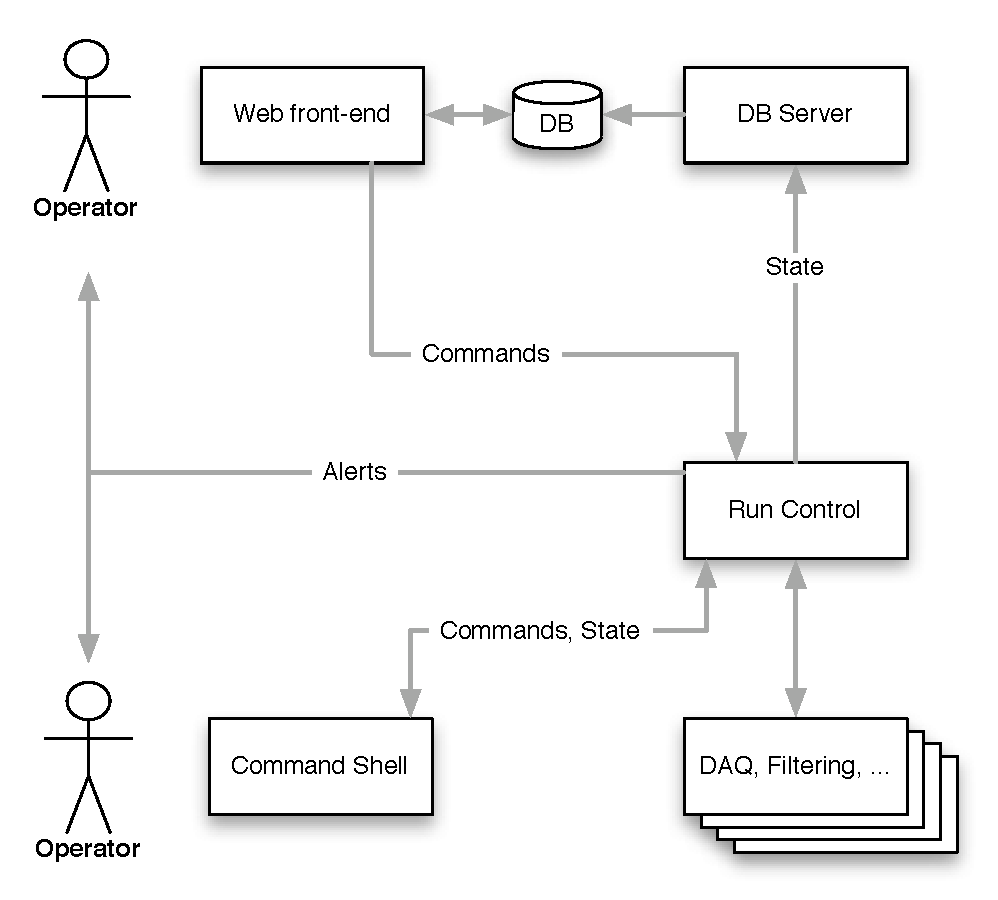
\includegraphics[width=80mm]{RCExpCont}
  \end{center}
    \caption[Run control system]{LBNE run control system design.}
  \label{fig:expcont}
\end{figure}

\subsubsection{Control and monitoring of LBNE components}

The run control system provides a control and monitoring
interface that can be integrated into each component.  This allows
operators to monitor and change the state (for example: Running,
Stopped, or Error) of each component.  This component control will be
available by both command line interface and graphical user web
interface.  This centralized control of all components that make up
DAQ systems will support complicated dependencies between components,
for example requiring that the DAQ be in a running mode before
starting a calibration system.

\subsubsection{Display of component monitoring and alerts}

During normal operation, all LBNE components will report system
monitoring and health values to the run control and will be
available for graphical display.  These values can include items such
as overall component health, trigger rates, memory buffer status or
rack temperatures.  These values will be archived in a database and be
presented in a detailed graphical user interface.  This interface can
be customized to the intended audience, with shift operator pages
presenting just high level status information, and expert views that
show detailed, per-channel information for use in detector debugging.

Historical views of component monitoring information will also be
available via the user interface.  This enables exploration of
historical reported information and correlation analysis between
detector components.  Detector components are not required to be under
\LBNE\ run control state control, but can simply report useful
information.  This type of reporting-only integration could
potentially be useful for offline systems, and would allow the
creation of a more complete historical view of detector history, with
information from data collection displayed side-by-side with
information from offline data analysis.

The \LBNE\ run control can also generate alerts to detector
operators and/or component experts if reported monitoring information
is outside expected ranges or a system component is in an error state.
These alerts can take any form (email, SMS, etc) and will be a unified
mechanism for alerting operators/experts of operational issues.

\subsubsection{Manage per-run information}

Run control is responsible for assigning a
unique number to each segment of data collected by data acquisition
systems (commonly referred to as a run number), as well as collecting
all user settings selected for a run.  This information will include
identifiers for the configurations used, components selected for operation
during a run, and any provided operator comments.  This information
will be stored in a database, and made available for
collaboration-wide use in online and offline analysis processes.

\subsubsection{Technology}
The run control uses several standard network and
web technologies.  These include:
\begin{itemize}
\item{XML-RPC - A remote procedure calling library using XML
    formatted messages to issue commands to remote processes, allowing
    the run control server to remotely control components}
\item{JSON - An open standard for message formatting that allows
    arbitrary data to be packaged in a human-readable format using
    name-value pairs for transmission.  Used by the run control
    components to format and send arbitrarily complex monitoring
    records.}
\item{ZeroMQ - A high performance message transport system that allows
    a large number of clients to report information to the run control
    server.}
\item{DJANGO - A graphical web content framework that can easily query
    and display information from database records.  The run control server
    stores recorded monitoring information in database tables, which
    are available for graphical presentation within the web-base user
    interface.}
\end{itemize}
While these technology choices are selected for their robust designs,
the modular design of the LBNE run control system allows for
flexibility in utilizing other technologies as replacements.

%%%%%%%%%%%%%%%%%%%%%%%%%%%%%%%%%%%%%%%%%%%%%%%%%%%%%%%%%%%%%%%%%%%%%%%%
%%%%%%%%%%%%%%%%%%%%%%%%%%%%%%%%%%%%%%%%%%%%%%%%%%%%%%%%%%%%%%%%%%%%%%%%
\section{Online Monitoring}
\label{sec:daq_om}

Rapid access to the data during data collection will be provided from
the artDAQ framework and used for making online monitoring histograms
and event display.  The online monitoring histograms will be used to
display the performance of the detector including e.g.\ noise rates,
dead channels and the online drift velocity measurement.  A framework
based on the ATLAS LHC experiment online monitoring will be used to
display the histograms, and associated historical data.  Since the
data are presented in the ART framework online, the development of new
histograms can be easily made offline first.

%%%%%%%%%%%%%%%%%%%%%%%%%%%%%%%%%%%%%%%%%%%%%%%%%%%%%%%%%%%%%%%%%%%%%%%%
%%%%%%%%%%%%%%%%%%%%%%%%%%%%%%%%%%%%%%%%%%%%%%%%%%%%%%%%%%%%%%%%%%%%%%%%
\section{Slow Control Systems }
\label{sec:daq_slowcontrol}

\subsection{Monitoring}

The slow controls system will allow monitoring of data both within and
outside the normal data taking.  The central server is based on the
same infrastructure as the run control described in
section~\ref{sec:daq_runcontrol}.  It will accept individual ZeroMQ
messages from sub-system components containing measurement readings
and will store them in a database on a server at the far detector.
This database will be replicated to a server at Fermilab which will
allow access via the standard offline interface being developed at
Argonne National Lab, based on the NOvA database system.

The slow control will generate status and historical plots of the
monitored values on demand from the run control Django system so that
shift-takers and experts can access the information easily through
the same framework as the run control.  Alarms will be used to
indicate to shift-crew and notify experts of values which are beyond
their normal range.

Several example data collection routines which send the zeroMQ message
to the central control will be provided, e.g. for the Wiener power
supplies, the rack protection units, the SSP monitoring functions, the
GPS time synchronisation and the aTCA crate managers.  Storage of
performance parameters derived from inside artDAQ, or from the data
analysis in the trigger or the online monitoring will also be reported
by zeroMQ messages to the slow control infrastructure.  Collaborators
who supply non-standard equipment will be able to provide their own
software to send the zeroMQ messages.  A centralized program will
harvest read-only data about the cryogenics and about the beam at
Fermilab which will also be available for status and historical
display.  All this data will be replicated to Fermilab and accessible
offline through the \LBNE\ offline database framework as described
above.

\subsection{Control}

The control functions of the \LBNE\ slow control will allow experts to
power off/on crates and racks remotely, for maintenance out-of hours
for attempts to restart the experiment after a crash when there is
no one with DAQ expertise present underground.  The rack protection
system will automatically (independently of the slow controls) shut
down electronics if a smoke, over-temperature or absence of cooling
condition is detected.  The slow controls will provide the interface
to setup the rack protection thresholds and to send reset commands
after a trip.

The slow control will have no control (only display of harvested
monitoring data) for the cryogenic system and the beam line at Fermilab.

%%%%%%%%%%%%%%%%%%%%%%%%%%%%%%%%%%%%%%%%%%%%%%%%%%%%%%%%%%%%%%%%%%%%%%%%
%%%%%%%%%%%%%%%%%%%%%%%%%%%%%%%%%%%%%%%%%%%%%%%%%%%%%%%%%%%%%%%%%%%%%%%%
\section{Interface with offline computing}
\label{sec:daq_offline}

As described in section~\ref{sec:daq_slowcontrol}, the interface to
the slow control monitoring data will be by a replication of the
online slow control database tables to Fermilab where they are
accessible via the standard database access tools developed for
\LBNE.  This method will also be used to give access to the run logging
database table which gives information about each run.  The values of
parameters used to configure at the start of each run will also be
stored in database tables and made available by this route. [The full
configuration files for each run will be backed up, and a separate job
will harvest the relevant ones (some are `plumbing parameters' used
for setting registers used only for lab debugging of the module)].

The default output format for artDAQ is readable by the art framework
directly.  As described in section~\ref{sec:daq_upper}, the data will be
stored briefly at each \COMPARTMENT\ and then a merging job will form
complete `runs' corresponding to all the data in the entire detector
for a given running period.  This will be archived to Fermilab, recorded in the
run control database and accessible directly by the offline
reconstruction and analysis programs.

%%%%%%%%%%%%%%%%%%%%%%%%%%%%%%%%%%%%%%%%%%%%%%%%%%%%%%%%%%%%%%%%%%%%%%%%
%%%%%%%%%%%%%%%%%%%%%%%%%%%%%%%%%%%%%%%%%%%%%%%%%%%%%%%%%%%%%%%%%%%%%%%%
\section{DAQ Infrastructure }
\label{sec:daq_infrastructure}

\subsection{Wide Area Network}

As in the case of MINOS and NO$\nu$A, it is expected that event data
can be transmitted over the network to Fermilab.  Although rates for
events of interest are comparable, data throughput for the \LBNE\
LArTPC is expected to be at least an order of magnitude higher.  A
bundle of single-mode fibers (latest estimate a 96 fiber bundle)
should be sufficient for transmitting the data from all four 10kT
modules to the surface, for transmitting the GPS synchronisation
(independently for the four 10kT modules) underground and to allow
expansion capacity.

\subsection{Online Data Storage}

To protect against significant periods of absent network connectivity,
it is desired to store a significant amount of the data emerging from
the DAQ to local storage.  A local data storage facility of $\sim
100\,$TB is expected to be more than adequate for five days worth of
detector data, even without prescaling cosmic-ray muon events.  This
storage is provided by a RAID disk array on one of the computing nodes
in the trigger farm.

\subsection{Power and Cooling}

Power and cooling requirements for the DAQ system described here are
fairly modest.  COB modules operate at around 100W each and the
commodity computers for the data collection and triggering at around
200W each.  More detailled power measurements will be provided by the
35t test to refine these numbers and add the other electronics
components into the estimate.

%%%%%%%%%%%%%%%%%%%%%%%%%%%%%%%%%%%%%%%%%%%%%%%%%%%%%%%%%%%%%%%%%%%%%%%%
%%%%%%%%%%%%%%%%%%%%%%%%%%%%%%%%%%%%%%%%%%%%%%%%%%%%%%%%%%%%%%%%%%%%%%%%
\section{Modular DAQ design}
\label{sec:daq_upper}

The modular DAQ design concept described here allows the
\COMPARTMENTS\ of the experiment to have semi-independent and
autonomous data taking --- essentially each \COMPARTMENT\ has sufficient
components (timing system, readout of detectors, data storage and
database storage) to run on its own, including having an independent
run-control state.  The modular DAQ design allows the whole detector to
be monitored and controlled as a single big detector, for simplicity
in operation.  It also allows triggers in one \COMPARTMENT\ to initiate
data collection in the other \COMPARTMENTS.
This strategy addresses the problem of ensuring that the possibility
of a supernova occurring while data is not being collected is very
close to zero, as long as power is present
underground.  It leverages the inherent redundancy, without
increasing cost, in the modular nature of the experiment.
It also has benefits in staging and allowing different \COMPARTMENTS\ 
to have different readout features.

The essential difference between this and having a single data
acquisition for the entire far detector is that if one \COMPARTMENT\
needs maintenance, or if the data collection stops due to a
communication problem or other reason, the other \COMPARTMENTS\ will
continue data collection uninterrupted.  If the complete detector is
not in data taking mode, this will be indicated on the operations
status and alarms screen and the operator will be able restart the
\COMPARTMENT\ and add it back into the overall run.  The run-log
database will indicate the periods when any compartment is missing
from the overall data collection.  It is felt that a mechanism by
which the entire detector does not stop data collection is essential
for a detector with the goal of collecting data from a
once-in-30-years supernova explosion event.  The modular DAQ design
concept will also improve overall uptime of the detector.

Each \COMPARTMENT\ runs as a separate data acquisition system with all
the real-time functions being capable of being run independently.
Each compartment has its own run-start and run-stop mechanisms (with a
standardized interface for initiating these commands and obtaining
state status information); its own timing system (required to be
synchronized to UTC to within 10$\mu$s, although it is likely with GPS
that a more stringent limits will be met by the individual
\COMPARTMENTS); its own data storage and data catalogue (with
a standard format for data and for indicating the period of collection
in each file).   Each \COMPARTMENT\ will also have its own independent
storage for slow control measurements.

A centralized `manager' for triggers across the entire detector will
be implemented.  This places a number of requirements on the readout
of the individual \COMPARTMENTS, although note that none of these is
more arduous than that required in order to collect beam spill data on
its own.  The \COMPARTMENTS\ are able to report when the activity it is
detecting warrants triggering of the adjacent (or all) \COMPARTMENTS,
which will be e.g.\ when a cosmic muon, atmospheric or beam neutrino
etc.\ is detected.  These are likely to only occur once every minute,
and a maximum acceptable rate at which a \COMPARTMENT\ should report
will be about one every five seconds.  The reports should arrive at
the central manager within 150\,ms of the event occurring.

The readout in the \COMPARTMENTS\ should be capable of storing the
complete set of signals for at least 200\,ms.  The central manager
will report back to the \COMPARTMENTS\ within this time any requests
from adjacent \COMPARTMENTS\ to collect data within a certain period.
The central manager will also distribute the spill timing from the
Fermilab LBNF beam to the \COMPARTMENTS.  It is likely that the
communication between the \COMPARTMENTS\ and the central manager are
implemented with a dedicated Ethernet network which is not used for any
other traffic.  The connection setup
will be for the individual \COMPARTMENT\ to subscribe to the central
management service, that way if the central management is not present
or stops, the \COMPARTMENT\ can run independently (although, of course,
it will not receive trigger requests from the other \COMPARTMENTS\ in
this case).  It is possible that an alternative way for a \COMPARTMENT\
to obtain the spill timing information independently of the central
manager may be available.

The run control will consist of a dedicated run-control for each
\COMPARTMENT\ which permits run-starts, -stops, monitoring, logging,
run-mode selection and configuration.  These run-controls can have
functions which vary between \COMPARTMENTS, but will conform to a
standard overall scheme to allow the operator to use a unique
interface (i.e.\ accessible from one web-page) to control and monitor
the entire experiment.  There will be a separate section of the
run-control which will give the overall status of the \COMPARTMENTS\ as
a whole.  It will be regarded as a fault situation unless all
\COMPARTMENTS\ are taking data in production configurations. 

The above parts of the modular DAQ design (the centralized manager and
the ability for the run-control to treat the \COMPARTMENTS\ as
autonomous, with an additional overall status) are all that is needed
in the real-time part of the DAQ subsystem.  The second part of the
modular DAQ design runs offline, shortly after the data collection has been
completed.  This part operates as a batch system on a farm of
computers and combines the data from the individual \COMPARTMENTS\
(which will have data files spanning different periods of time) into
a single sequence of time-ordered files for archival and production
use offline.  The beam line status and monitoring data will be
transferred from Fermilab and incorporated into the files as well
(essentially being regarded as an additional pseudo-\COMPARTMENT).
